\chapter{Kiến thức nền tảng} \label{Chapter2}
\noindent Ở chương này, khóa luận sẽ trình bày các khái niệm xoay quanh hệ thống gợi ý, những hướng tiếp cận chính khi ta nghĩ đến việc xây dựng một hệ thống giúp người dùng có thể dễ dàng hơn cho việc lựa chọn sản phẩm, làm rõ hơn những vấn đề mà những công trình nghiên cứu từ trước đến nay vẫn còn gặp phải. Bên cạnh đó, mạng hoc sâu đồ thị cũng được nhắc đến, mọi tương tác giữa người dùng và sản phẩm đều được biểu diễn dưới dạng đồ thị. Đặc biệt, ta sẽ đề cập thẳng tới ``Học tự giám sát'' - một mô hình học đã áp dụng rất thành công trên dữ liệu dạng hình ảnh, lý giải được tại sao nó lại nhận được rất nhiều sự quan tâm gần đây. Toàn bộ những kiến thức này sẽ cung cấp cho người đọc một nền tảng tốt từ đó hiểu rõ được hiệu quả mà học tự giám sát mang lại cho hệ thống gợi ý.

\section{Hệ thống gợi ý}

\subsection{Hệ thống gợi ý là gì?}

\noindent Con người luôn mong muốn được trải nghiệm một không gian được cá nhân hóa hay là giảm bớt gánh nặng trong việc suy nghĩ lựa chọn. Xã hội ngày càng phát triển, điều đó luôn kéo theo sự đòi hỏi về nền tảng công nghệ thông tin cũng phải đi lên. Để đạt được những điều đó, hệ thống gợi ý đã ra đời và đang ngày càng được phát triển. Hệ thống gợi ý được sinh ra với khả năng hỗ trợ con người trong việc ra quyết định, cung cấp cho họ các gợi ý về những sản phẩm mà họ có thể cần.

Nói qua về ý tưởng của hệ thống gợi ý. Hệ thống gợi ý giúp giảm bớt thời gian, công sức cho việc đánh giá mức độ ưa thích của người dùng đối với một sản phẩm mà họ chưa từng được tiếp cận. Mức độ yêu thích được thể hiện qua điểm xếp hạng (rating) đối với sản phẩm đó. Trước khi vào chi tiết, ta có thể hiểu đơn giản, những điểm xếp hạng chưa biết tới có thể được dự đoán bằng cách dựa vào điểm xếp hạng mà người dùng này đánh giá trên các sản phẩm khác, những sản phẩm mà người dùng đã tiếp cận và còn dựa vào một số thông tin được mô tả. Khi đó, ta có thể ước tính được điểm xếp hạng cho các sản phẩm mà ta chưa biết đến, từ đó đề xuất cho người dùng nhóm những sản phẩm có rating ước tính cao nhất \cite{survey:sota-rec-system}. Một ví dụ về tương tác đánh giá có thể biểu diễn dưới dạng một ma trận tiện ích -- \textit{Utility matrix}.

Trong bài toán hệ thống gợi ý, ta quan tâm đến hai thực thể là người dùng (user) và sản phẩm (item). Sản phẩm hiểu đơn giản là những thứ mà người dùng có thể `tiêu thụ' được như hàng hóa, phim, bài hát,... Khi người dùng tiếp cận tới các sản phẩm, người dùng sẽ luôn thể hiện mức độ quan tâm của riêng mình đối với các sản phẩm đó. Để thể hiện mức độ quan tâm của người dùng đến sản phẩm, ta sẽ sử dụng đến ratings. Tập hợp các ratings tạo thành một ma trận tiện ích, qua những giá trị này, ta có thể biết được mức độ yêu thích của một người dùng đối với sản phẩm. Trong ma trận tiện ích, phần lớn sẽ tồn tại rất nhiều khoảng trống, ta gọi những trường hợp này là ma trận thưa (sparse matrix). Những khoảng trống này ngụ ý rằng, ta không có thông tin rõ ràng về mức độ yêu thích của người dùng đối với sản phẩm đó.

\begin{table}[H]
    \centering
    \begin{tabular}{|l|l|l|l|l|}
        \hline
             & A & B & C & D \\ \hline
        Pop  & 3 & 5 &   & 1 \\ \hline
        Rock &   & 8 & 3 &   \\ \hline
        R\&B & 1 &   &   &   \\ \hline
        Jazz &   &   & 1 &   \\ \hline
    \end{tabular}
    \caption{Ví dụ một ma trận tiện ích}
    \label{table:utility-matrix}
\end{table}

Ví dụ với ma trận tiện ích trên, ta thấy được mức độ yêu thích của mỗi người dùng đối với các thể loại nhạc Pop, Rock, Jazz,... trên thang điểm $0-10$. Những điểm không có giá trị là do ta không có thông tin về mức độ yêu thích của người dùng đối với những sản phẩm trên, ta cần tìm hay dự đoán những giá trị đó.

Việc dự đoán các giá trị còn thiếu này có thể thực hiện bằng cách sử dụng các phương pháp học máy, lý thuyết gần đúng hoặc bằng các phương pháp phỏng đoán khác nhau. Tổng quát lại, ta có thể thực hiện thực hiện bằng hai cách. Cách thứ nhất ta sẽ dựa vào các heuristic để định nghĩa các utility function (hàm tiện ích) và đo lường hiệu quả của nó. Ví dụ như ta có thể đề xuất cho người dùng những bộ phim mà có thể loại, đạo diễn hay diễn viên mà người dùng đánh giá cao trước đó. Cách thứ hai là người dùng dựa vào các utility function để tối ưu dựa trên một tiêu chí nào đó như Mean Square Error,... Khi đã hoàn tất việc dự đoán các ratings, nhiệm vụ đề xuất các mặt hàng cho người dùng được thực hiện bằng cách chọn một hoặc nhiều mặt hàng có điểm rating cao nhất trong số sản phẩm ta cần dự đoán. Đương nhiên là trên thực tế, không phải lúc nào ta cũng có tiếp cận với một bộ dữ liệu đầy đủ và có thể biểu diễn được dưới dạng ma trận tiện ích. Cùng với những hạn chế của hệ thống gợi ý mà sẽ được đề cập sau, ta cần phải có những cách tiếp cận thông minh hơn.

Hiện tại, với bài toán hệ thống gợi ý, ta có 3 hướng tiếp cận chính \cite{survey:sota-rec-system} là Content-based, Collaborative filtering, và Hybrid filtering. Ta sẽ không đi giải thích quá sâu về các hướng tiếp cận mà chỉ mô tả các ý tưởng chính.

\subsection{Các hướng tiếp cận phổ biến trong bài toán Hệ thống gợi ý}

\subsubsection{Content-based systems}
\noindent Hệ thống gợi ý dựa trên nội dung -- Content-based system \cite{content-based-rec} là một trong những phương pháp chung cho bài toán gợi ý. Ở hướng tiếp cận này, ta sẽ giới thiệu những sản phẩm mới cho người với điều kiện là chúng tương tự với những sản phẩm mà chính người dùng đã đánh giá cao trước đó. Ví dụ, khi đề xuất phim ở trên Netflix, hệ thống gợi ý sẽ tìm ra những điểm tương đồng chung của những bộ phim mà người dùng đã xem trước đó (đạo diễn, diễn viên, thể loại,...) từ đó chỉ ra được những phim có độ tương đồng cao (nhất) với những phim đã người dùng đã từng xem.

Cụ thể hơn, với mỗi sản phẩm ta sẽ xây dựng một ``profile'' đại diện cho các đặc trưng quan trọng của sản phẩm dưới dạng một vector đặc trưng. Ví dụ về các đặc trưng như thể loại, chủ đề, nhạc sĩ, ca sĩ (lĩnh vực âm nhạc); thiết kế, công dụng, phân khúc giá (sản phẩm hàng tiêu dùng). Một ví dụ nữa, khi xây dựng các vector đặc trưng cho văn bản, ta có thể sử dụng TF-IDF (Term Frequency - Inverse Document Frequency) để chọn ra những từ quan trọng và vector đặc trưng cũng được xây dựng dựa vào đó.

``Profile'' của người dùng đại diện cho những thị hiếu và sở thích của người dùng. Để gợi ý cho người dùng những sản phẩm mới, ta có thể sử dụng độ tương đồng cosine \cite{cos-sim} để đo mức độ tương đồng giữa người dùng và sản phẩm cần dự đoán.
\begin{equation}
    s(q, w) = \cos{\widehat{(q, w)}} = \frac{q^T w}{||q|| \cdot ||w||},
    \label{eq:cosine-sim}
\end{equation}
với $q$ và $w$ là hai vector cùng kích thước mô tả đặc trưng của người dùng/sản phẩm, $\widehat{(q, w)}$ là góc giữa hai vector đó.

Từ những khái niệm trên, ta thấy với cách tiếp cận này ta hoàn toàn không phụ thuộc dữ liệu từ những người dùng khác, mọi thứ phụ thuộc vào chính bản thân chúng ta. Đặc biệt, bằng cách sử dụng cách này, ta có thể nhận được gợi ý những sản phẩm mới được vào hệ thống hoặc những sản phẩm không phổ biến dựa trên những thuộc tính, đặc trưng của sản phẩm đó. Tuy nhiên với những người mới mới tiếp cận dịch vụ, sẽ rất khó nếu không rõ sở thích/thị hiếu của người dùng. Bên cạnh đó, ta nhận ra, ta cũng không thể khám phá ra những sở thích còn tiềm ẩn của người dùng.

\subsubsection{Collaborative filtering}
\noindent Hệ thống gợi ý sử dụng lọc cộng tác -- Collaborative filtering \cite{survey:CF-tech}. Với hướng tiếp cận này, thay vì phu thuộc hoàn toàn vào đặc trưng của các sản phẩm mà người dùng đã đánh giá trước đó, ta sẽ dựa trên hành vi của nhiều người dùng khác lên một sản phẩm để dự đoán mức độ quan tâm của người dùng lên sản phẩm đó dựa trên một độ đo sự tương đồng. Người ta thường sử dụng độ tương đồng cosine (Cosine similarity) để đo mức độ ``gần nhau'' giữa các người dùng/sản phẩm. Khác với Content-based, ta sẽ đo mức độ tương tự giữa người dùng hoặc giữa sản phẩm với nhau. Thông tin trích ra được và có thể học được từ cách tiếp cận này còn gọi là tín hiệu collaborative filtering.

Ở hướng này, ta có thể khai thác theo kiểu người dùng -- người dùng hoặc sản phẩm -- sản phẩm. Ví dụ với người dùng -- người dùng, người dùng A thích các thể loại nhạc Pop, R\&B và Jazz, người dùng B thì thích các thể loại Pop, R\&B thì khả năng cao là người dùng A cũng thích nhạc Jazz như người A. Ví dụ với sản phẩm -- sản phẩm, ta có thể dự đoán độ yêu thích của người dùng với bộ phim Harry Potter 7 dựa trên mức độ yêu thích của họ cùng với những người dùng khác lên các phim Harry Potter. Thông thường cách làm này mang lại hiệu quả tốt hơn so với người dùng -- người dùng vì người dùng luôn đa dạng sở thích (có rất nhều sở thích tiềm ẩn).

Bằng cách này, ta sẽ phụ thuộc vào tương tác của những người dùng khác trong toàn bộ không gian tương tác. Ta cũng có thể nhận được sản phẩm nằm ngoài sở thích (đã bộc lộ) của mình. Tuy nhiên việc gợi ý sẽ không hiệu quả nếu ta không có số lượng tương tác giữa người dùng và sản phẩm đủ lớn. Ta cũng khó nhận được sản phẩm mới đưa vào hệ thống gợi ý.

Ngoài Content-based và Collaborative filtering ta còn có phương pháp kết hợp giữa hai hướng tiếp cận này gọi là hybrid filtering. 

\subsection{Vấn đề của hệ thống gợi ý} \label{2.1.3-rec-issues}

\noindent Hệ thống gợi ý không mới nhưng vẫn còn rất nhiều vấn đề tồn tại từ lâu nhưng vẫn luôn là chủ đề nóng cần phải giải quyết \cite{survey:rec-sys-tech&issues}:

\begin{itemize}
    \item[(1)] \textbf{Dữ liệu thưa}: Dữ liệu thưa hiểu nôm na là dữ liệu có rất nhiều giá trị bằng 0/null (khác với dữ liệu bị thiếu). Trong ngữ cảnh của hệ thống gợi ý, người dùng có khuynh hướng chỉ tương tác với một phần rất nhỏ trong cơ sở dữ liệu của hàng triệu các sản phẩm, các tương tác này có thể được coi như là dữ liệu có giá trị khác 0/null và các tương tác không tồn tại với các sản phẩm khác sẽ được coi như là có giá trị 0/null. Vậy nên việc tìm ra nhiều người dùng mà có lịch sử tương tác giống nhau, hay việc phân tích tương tác của người dùng đối với một tập sản phẩm nhất định là rất khó.\\
    Vì sự khó khăn về việc tìm hành vi giống nhau của người dùng và phân tích hành vi nên dữ liệu thưa là một vấn đề lớn để đưa ra dự đoán về tương tác của người dùng một cách đáng tin cậy. Đối với hệ thống gợi ý thì hiệu năng của nó bị ảnh hưởng một cách đáng kể.
    
    \item[(2)] \textbf{Sự thay đổi hành vi người dùng}: Sở thích và hành vi của người dùng không cố định và thường thay đổi rất nhanh theo thời gian và tùy vào nhiều trường hợp và các yếu tố khác nhau như yếu tố mùa vụ, xu hướng. Rating của người dùng chỉ mang tính nhất thời tại một thời điểm và bị nhiều yếu tố tác động.
    
    \item[(3)] \textbf{Sự riêng tư của người dùng}: Để có thể đưa ra các gợi ý phù hợp cho người dùng, hệ thống gợi ý cần khá nhiều thông tin về sở thích và lịch sử tương tác của họ. Có thể nói dữ liệu này rất nhạy cảm và mang nhiều rủi ro, có giá trị rất lớn và dễ là đối tượng cho tin tặc tấn công, hoặc bị bán cho các công ty quảng cáo. Trong khi đó, đa số người dùng thường không biết lượng thông tin mà họ cung cấp cho các hệ thống này lớn tới đâu, và không biết thông tin đó đang được dùng để làm gì.
    
    \item[(4)] \textbf{Cold Start}: Cold Start xảy ra khi ta không có đủ dữ liệu để có thể tìm ra được các liên hệ, các mối liên kết giữa người dùng và sản phẩm. Vấn đề này xảy ra trên cả người dùng và sản phẩm. Có các nguyên nhân chính dẫn đến vấn đề này như sau: hệ thống gợi ý, đánh giá chỉ vừa mới được khởi động; một người dùng hay sản phẩm mới được đưa vào hệ thống; một sản phẩm ít được tương tác/đánh giá hay một người dùng ít đánh giá/thể hiện mức độ yêu thích với các sản phẩm.
\end{itemize}

\section{Mạng học sâu đồ thị -- Graph neural network}
% [A Survey of Graph Neural Networks for Recommender Systems: Challenges, Methods, and Directions]
% [https://arxiv.org/pdf/2006.09963.pdf] Graph Pre-Training ở đây
% [Weisfeiler and Leman Go Neural: Higher-order Graph Neural Networks]

\noindent Dạo gần đây nổi lên rất nhiều công trình nghiên cứu về cấu trúc đồ thị và được áp dụng lên nhiều bài toán như mạng xã hội, mạng cấu trúc phân tử, hệ thống gợi ý. Sự phát triển này bắt nguồn từ các thành tựu mà mạng neuron tích chập (CNN) và học biểu diễn đồ thị (GRL) mang  lại. Khi áp dụng với ảnh hoặc văn bản, CNN mang lại hiệu quả rất tốt trong việc trích xuất đặc trưng. Tuy nhiên, hiện nay, có rất nhiều bài toán mà dữ liệu không thể biểu diễn được dưới dạng 1D, 2D như ảnh hay chữ cái. Người ta xếp chúng thuộc kiểu dữ liệu Non-Euclidean. Những dữ liệu kiểu như thế này ngày càng trở nên phổ biến trong thời gian gần đây bởi sự áp dụng rộng rãi trong nhiều lĩnh vực cuộc sống như những bài toán liên quan đến mạng xã hội, các bài toán liên quan liên kết giữa các phân tử, nguyên tử trong nghiên cứu thuốc. Với kiểu Non-Euclidean, ta luôn mong muốn tổng quát hóa được các đối tượng. Để giải quyết được các bài toán như vậy ta có thể sử dụng các thực thể đồ thị như node, cạnh,... Ở phần này ta sẽ đề cập đến những kiến thức chung nhất về mạng học sâu đồ thị -- Graph neural network (GNN) lẫn học biểu diễn đồ thị.

\subsection{Đồ thị là gì?}
\noindent Một đồ thị (graph) \cite{intro-graph-theory} là một cấu trúc toán học trừu tượng mà chứa một tập các vật thể gọi là đỉnh (vertex), còn có tên khác là node, và mối liên kết giữa các node đó. Nói rõ hơn là hai node (hoặc nhiều hơn) có thể có sự liên kết nào đó với nhau, những mối liên kết này được gọi là cạnh (edge).

\begin{figure}[H]
    \centering
    \begin{subfigure}[b]{0.42\textwidth}
        \centering
        \includesvg[scale=0.8]{images/Chapter2/graph_example.svg}
        \subcaption{Một đồ thị vô hướng.}
        \label{subfig:graph-example}
    \end{subfigure}
    \hspace{15mm}
    \begin{subfigure}[b]{0.42\textwidth}
        \centering
        \includesvg[scale=0.8]{images/Chapter2/graph_directed_example.svg}
        \subcaption{Một đồ thị có hướng.}
        \label{subfig:graph-directed-example}
    \end{subfigure}
    \caption{Ví dụ về đồ thị.}
\end{figure}

Dưới phương diện toán học, ta có thể định nghĩa một đồ thị bằng ký hiệu $G$, bao gồm tập node $V$ và tập $E$:
\begin{equation}
    G = (V, E),
\end{equation}
trong đó, $V = \{v_i \; | \; 0 \leq i < |V|\}$, $E = \{e_i \; | \; 0 \leq i < |E|\}$ với $|V|$ và $|E|$ lần lượt là kích thước của tập $V$ và $E$. Với ví dụ hình \ref{subfig:graph-example}, ta có đồ thị với tập node $V = \{v_0, v_1, v_2, v_3, v_4\}$ và tập cạnh $E = \{e_0, e_1, e_2, e_3, e_4\}$. Ngoài ra ta còn có thể biểu diễn một cạnh bằng cặp node mà nó kết nối, ví dụ $e_3 \equiv (v_2, v_3)$.

Có hai loại đồ thị cơ bản là đồ thị vô hướng (hình \ref{subfig:graph-example}) và đồ thị có hướng (hình \ref{subfig:graph-directed-example}). Đồ thị có hướng khác với đồ thị vô hướng ở chỗ là hai node có liên kết trong đồ thị có hướng có thứ tự, nghĩa là mỗi cạnh là một mũi tên với hướng đi ra từ một node và đi vào một node khác. Ngoài ra, tùy vào bài toán nhất định mà ta có thể biến đổi một đồ thị cơ bản thành những dạng đồ thị phức tạp hơn, mỗi node và cạnh có thể chứa thêm nhiều thông tin hơn. Cấu trúc đồ thị xuất hiện rất nhiều trong cuộc sống xung quanh ta, một số ví dụ là mạng lưới điện, bản đồ giao thông, quan hệ bạn bè, cấu trúc phân tử...

\begin{figure}[H]
    \centering
    \begin{subfigure}[b]{0.4\textwidth}
        \centering
        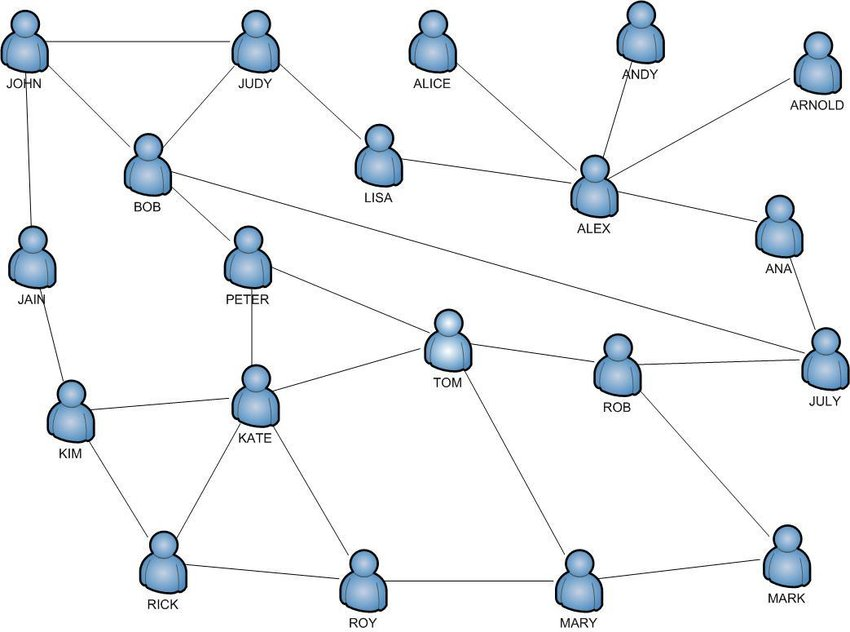
\includegraphics[scale=0.3]{images/Chapter2/friends-graph.png}
        \subcaption{Sơ đồ quan hệ.}
    \end{subfigure}
    \hspace{15mm}
    \begin{subfigure}[b]{0.4\textwidth}
        \centering
        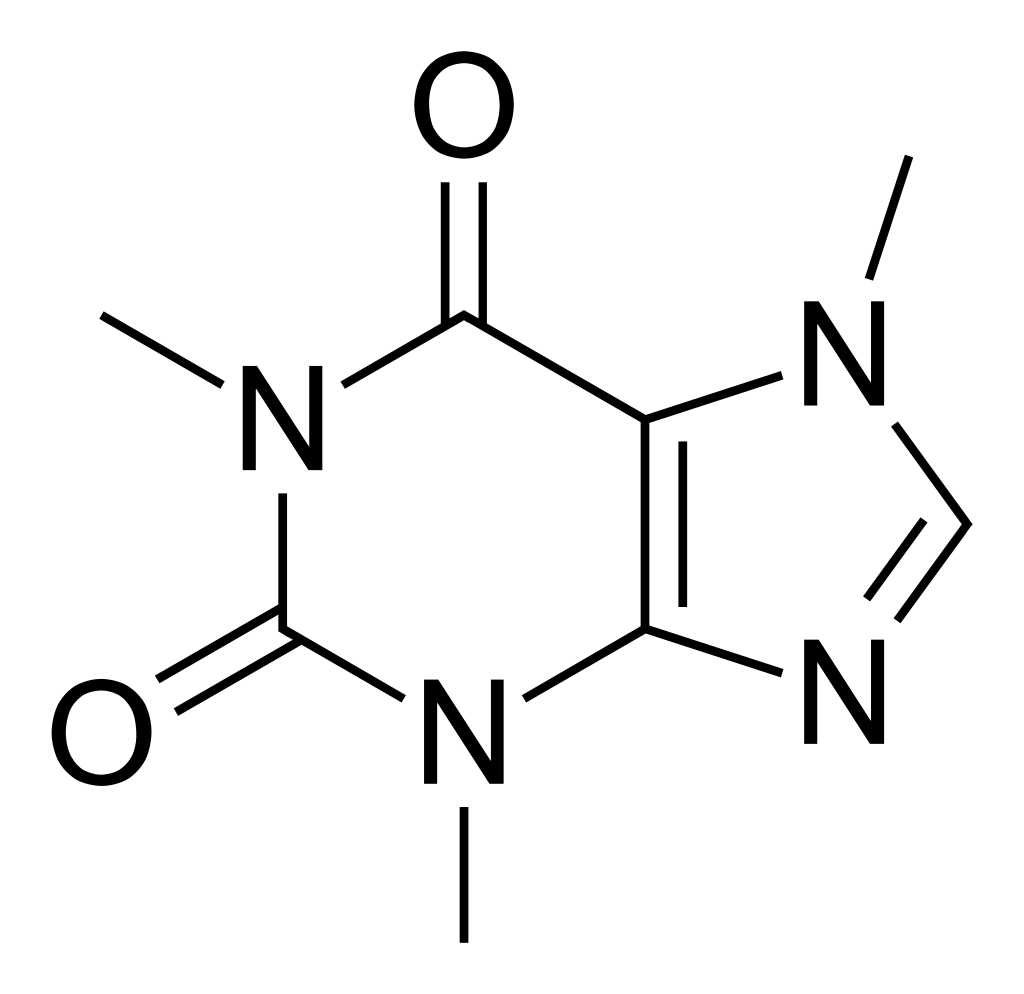
\includegraphics[scale=0.1]{images/Chapter2/caffeine_structure.png}
        \vspace*{8mm}
        \subcaption{Cấu trúc phân tử của caffeine.}
    \end{subfigure}
    \caption{Ví dụ về cấu trúc đồ thị trong thực tế.}
\end{figure}


\subsection{Các loại đồ thị}

\noindent Như đã nói, dữ liệu dạng đồ thị cũng có thể được biểu diễn dưới nhiều dạng khác nhau, khi thiết kế một mạng học sâu để giải quyết một bài toán dạng đồ thị thì cũng nên tìm hiểu kĩ và áp dụng kiểu đồ thị cho phù hợp với bài toán đó. Thông thường thì các model học trên đồ thị sẽ được thiết kế dựa trên tính liên kết có sẵn của dữ liệu rời rạc (VD. Dữ liệu cấu trúc như cấu trúc phân tử, đồ thị tri thức,...) hoặc bằng cách trìu tượng hóa dữ liệu chưa có cấu trúc nhất định (VD. Dữ liệu dạng văn bản trong đoạn văn,...). Theo thống kê của Zhou và đồng nghiệp \cite{review:GNN}, một đồ thị có thể được phân loại như sau:

\begin{itemize}
    \item \textbf{Directed/undirected graph (có hướng/vô hướng):} Như đã định nghĩa ở trên, đồ thị có hướng có nghĩa là thứ tự vào ra của cạnh là một thông tin mà đồ thị vô hướng không có, điều này có thể biểu diễn tính một chiều khi di chuyển từ node này sang node khác, ví dụ là với đường một chiều trong bản đồ giao thông; ngược lại, đồ thị vô hướng trong nhiều trường hợp lại phù hợp hơn cho việc tổng quát hóa vì mỗi cạnh của đồ thị vô hướng có thể hiểu là 2 cạnh có hướng ngược nhau.
    
    \item \textbf{Homogeneous/heterogeneous graph (đồng nhất/không đồng nhất):} Trong đồ thị đồng nhất, chỉ có 1 loại (type) node và cạnh; trong đồ thị không đồng nhất thì có thể có nhiều hơn 1 loại node và cạnh.
    
    \item \textbf{Static/Dynamic graph (tĩnh/động):} Đồ thị tĩnh có cấu trúc/đặc trưng không thay đổi theo thời gian và đồ thị động có cấu trúc/đặc trưng thay đổi theo thời gian.
\end{itemize}

\subsection{Thiết kế chung của mạng GNN} \label{2.2.3-GNN-design}
% [Graph neural networks: A review of methods and applications -- www.sciencedirect.com/science/article/pii/S2666651021000012]
% [A Comprehensive Survey on Graph Neural Networks -- ieeexplore.ieee.org/ielaam/5962385/9312808/9046288-aam.pdf]
% [Strategies for pre-training graph neural networks -- https://arxiv.org/pdf/1905.12265.pdf]
% [Data Augmentation for Deep Graph Learning: A Survey -- https://arxiv.org/pdf/2202.08235.pdf]
% [Weisfeiler and Leman Go Neural: Higher-Order Graph Neural Networks -- https://ojs.aaai.org/index.php/AAAI/article/download/4384/4262]
% [Neural Message Passing for Quantum Chemistry -- http://proceedings.mlr.press/v70/gilmer17a/gilmer17a.pdf]
\subsubsection{Xác định output}
\noindent Khi thiết kế mạng GNN thì ta cần phải xác định được tác vụ (task) của nó. Thông thường khi giải quyết bài toán học trên đồ thị thì có 3 loại tác vụ chính \cite{review:GNN, survey:GNN, survey:aug-for-dgl}:
\begin{itemize}
    \item \textbf{Node-level}: Là các tác vụ tập trung vào dự đoán các đặc trưng của node, ví dụ như phân lớp node, hồi quy, phân cụm...
    
    \item \textbf{Edge-level}: Là các tác vụ dự đoán các đặc trưng của cách cạnh như phân lớp và dự đoán liên kết giữa các node.
    
    \item \textbf{Graph-level}: Là các tác vụ dự đoán các đặc trưng của toàn bộ đồ thị như phân lớp, hồi quy và matching các đồ thị.
\end{itemize}
Tùy vào loại tác vụ nhất định, ta có thể thiết kế 1 hàm mất mát phù hợp. Ví dụ tác vụ phân lớp thì có thể dùng cross-entropy...

\subsubsection{Học biểu diễn} \label{2.2.2-reprensentation-learning}
\noindent Để sử dụng đồ thị trong các ứng dụng khai thác dữ liệu và học máy trong các tác vụ học và dự đoán, đồ thị và các thực thể của nó như nút và cạnh cần được biểu diễn bằng các đặc trưng dạng số. Một trong những cách phổ biến là biểu diễn đồ thị bằng ma trận kề. Tuy nhiên, việc biểu diễn ma trận kề lại tốn khá nhiều bộ nhớ, đặc biệt là với các đồ thị lớn. Một tiếp cận thay thế là trích xuất đặc trưng, ví dụ dựa vào các đặc điểm như bậc (degree), hệ số phân cụm (clustering coefficient), kernel functions,... Tuy nhiên điều này khá hạn chế về mặt thời gian và khó để bắt kịp các tiến trình học. Học biểu diễn (Representation learning) \cite{survey:graph-rep-learning} là giải pháp cho vấn đề vừa nêu trên bằng cách tự động sinh ra các vector biểu diễn cho đồ thị.

% A Survey on Graph Representation Learning Methods (SHIMA KHOSHRAFTAR and AIJUN AN, Electrical Engineering and Computer Science Department, York University, Canada)

\begin{figure} [H]
    \centering
    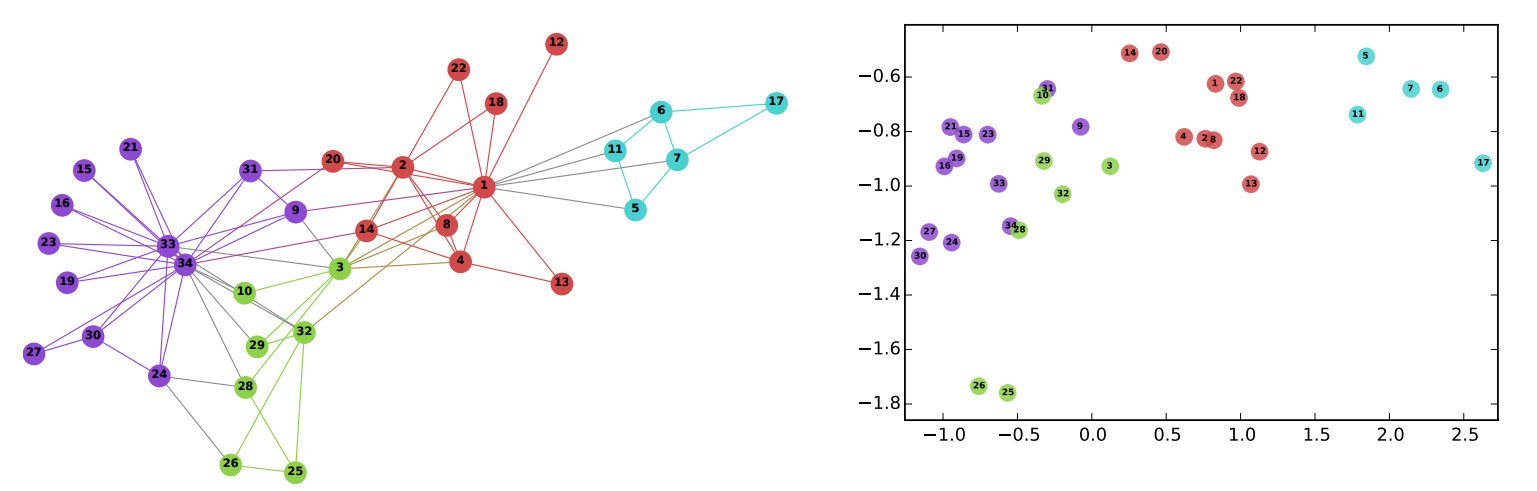
\includegraphics[scale=0.35]{images/Chapter2/node-embedding.png}
    \caption[Ví dụ về node embedding.]{Ví dụ về node embedding. Bên trái là đồ thị gốc, bên phải là biểu diễn của đồ thị trong không gian embedding (Hình ảnh trích từ bài báo của Khoshraftar \cite{survey:graph-rep-learning}).}
    \label{fig:node-embed-example}
\end{figure}

Ý tưởng của \textbf{học biểu diễn} là nhúng một phần hoặc cả đồ thị vào một không gian vector. Mối quan hệ hình học trong không gian này vẫn thể hiện được cấu trúc của đồ thị gốc. Hình \ref{fig:node-embed-example} là một ví dụ về node embedding. Điểm tương đồng giữa các vector embedding của các node cũng thể hiện được sự tương đồng giữa các node trong đồ thị. Điều này cũng đúng với mối liên hệ giữa các cạnh hay là mối liên hệ giữa các đồ thị con trong đồ thị gốc. Giờ đây, các embedding này có thể được sử dụng để làm input cho các tác vụ downstream.

\subsubsection{Quá trình tích chập trên đồ thị -- Neighborhood aggregation/Message passing}

\begin{figure}[H]
    \centering
    \scalebox{.9}{
        \begin{tikzpicture}[
            vertex/.style = {circle, draw, inner sep=4pt, fill=white},
            red/.style = {vertex, fill=fireenginered},
            orange/.style = {vertex, fill=cadmiumorange},
            blue/.style = {vertex, fill=airforceblue},
            green/.style = {vertex, fill=asparagus},
            purple/.style = {vertex, fill=darklavender},
            cyan/.style = {vertex, fill=electriccyan!80!black},
            yellow/.style = {vertex, fill=goldenyellow},
            ]
            \node[red]      (A) at (5, 1.5) {};
            \node[orange]   (B) at (3, 3) {};
            \node[blue]     (C) at (2, 1.5) {};
            \node[green]    (D) at (4.5, 0) {};
            \node[purple]   (E) at (6, 1) {};
            \node[cyan]     (F) at (6.5, 2.5) {};
            \node[yellow]   (G) at (6.1, 0.2) {};
    
            \node[red, inner sep=6pt]       (A1) at (9, 1.5) {};
            \node[orange, inner sep=6pt]    (B1) at (15, 3) {};
            \node[green, inner sep=6pt]     (D1) at (15.2, 1.5) {};
            \node[purple, inner sep=6pt]    (E1) at (15, 0) {};
            
            \node[draw=gray, fill=gray!30, fit={(10, 0.75) (13, 2.25)}, inner sep=0pt, text height=0.6cm] (NA) {\small Neighborhood\\aggregation};
            
            \node[draw=gray, fill=gray!30, fit={(16, 1) (16.5, 2)}, inner sep=0pt, rotate around={23.5:(-4.75, 0)}] (NA1) {};
            \node[draw=gray, fill=gray!30, fit={(16, 1) (16.5, 2)}, inner sep=0pt] (NA2) {};
            \node[draw=gray, fill=gray!30, fit={(16, 1) (16.5, 2)}, inner sep=0pt, rotate around={-23.5:(-4.75, 0)}] (NA3) {};
    
            \node[red, inner sep=6pt]       (A2) at (16.7, 4.5) {};
            \node[blue, inner sep=6pt]      (C2) at (17.3, 3.3) {};
            \node[green, inner sep=6pt]     (D2) at (17.2, 4) {};
    
            \node[red, inner sep=6pt]       (A3) at (17.5, 2) {};
            \node[orange, inner sep=6pt]    (B3) at (17.5, 1) {};
    
            \node[red, inner sep=6pt]       (A4) at (17.3, -0.3) {};
            \node[cyan, inner sep=6pt]      (F4) at (16.7, -1.5) {};
            \node[yellow, inner sep=6pt]    (G4) at (17.2, -1) {};
            
            \draw[gray, thick]
                (A) -- (B)
                (B) -- (C)
                (A) -- (D)
                (B) -- (D)
                (A) -- (E)
                (E) -- (F)
                (E) -- (G);
    
            \draw[draw, very thick, -latex] (NA) -- (A1);
            \draw[gray, very thick, dotted, -latex] (B1) -- (NA);
            \draw[gray, very thick, dotted, -latex] (D1) -- (NA);
            \draw[gray, very thick, dotted, -latex] (E1) -- (NA);
            \draw[draw, very thick, -latex] (NA1) -- (B1);
            \draw[gray, very thick, dotted, -latex] (A2) -- (NA1);
            \draw[gray, very thick, dotted, -latex] (C2) -- (NA1);
            \draw[gray, very thick, dotted, -latex] (D2) -- (NA1);
            \draw[draw, very thick, -latex] (NA2) -- (D1);
            \draw[gray, very thick, dotted, -latex] (A3) -- (NA2);
            \draw[gray, very thick, dotted, -latex] (B3) -- (NA2);
            \draw[draw, very thick, -latex] (NA3) -- (E1);
            \draw[gray, very thick, dotted, -latex] (A4) -- (NA3);
            \draw[gray, very thick, dotted, -latex] (F4) -- (NA3);
            \draw[gray, very thick, dotted, -latex] (G4) -- (NA3);
            
        \end{tikzpicture}
    }
    \caption{Ví dụ về quá trình tích chập trên đồ thị}
\end{figure}

\noindent Ta có $G = (V, E)$ là đồ thị với tập node $V$ và tập cạnh $E$, $\mathbf{e}_v^{(0)}$ là embedding ban đầu của node $v \in V$, $\mathbf{h}_{uv}$ là embedding của cạnh $(u, v) \in E$, và $\mathcal{N}_v$ là tập các node có cạnh nối với $v$.

Tương tự như một model CNN, trong đó giá trị tích chập của một phần tử trong tensor ở một lớp (layer) là tổ hợp tuyến tính của một nhóm phần tử lân cận với phần tử đó từ lớp trước, một model GNN cơ bản cũng có một mô hình tích chập riêng gọi là Neighborhood aggregation (tổng hợp láng giềng), hay có một tên khác là Message passing (truyền tin) \cite{messagepassing-quantum-chemistry}, trong đó, embedding của node $v$ sẽ được cập nhật (combine) thông qua embedding tổng hợp của các node $u$ nối với $v$ thông qua cạnh $(u, v)$ sử dụng một hàm tổng hợp (aggregate). GC \cite{GC-model}, GG-NN \cite{GG-NN}, GraphSAGE \cite{GraphSAGE} là một số model GNN đời đầu áp dụng phương pháp này.

Thông thường thì phép tích chập này tại lớp thứ $l$ của GNN có biểu diễn toán học \cite{review:GNN, survey:aug-for-dgl, strat-pretrain-GNN, higher-order-GNN} như sau:
\begin{equation}
    \mathbf{e}_v^{(l)} = f_{\text{combine}}^{(l)}(\mathbf{e}_v^{(l-1)}, f_{\text{aggregate}}^{(l)}(\{(\mathbf{e}_v^{(l-1)}, \mathbf{e}_u^{(l-1)}, \mathbf{h}_{uv}) | u \in \mathcal{N}_v\})),
\end{equation}
trong đó, $f_{\text{aggregate}}^{(l)}(\cdot)$ là hàm tổng hợp các node và cạnh lân cận, và có một số lựa chọn như là Mean, Weighted sum \cite{GIN}, LSTM \cite{GraphSAGE}. $f_{\text{combine}}^{(l)}(\cdot)$ là hàm cập nhật embedding của node tại lớp thứ $l$, một lựa chọn phổ biến được để xuất bởi Hamilton và cộng sự \cite{GraphSAGE} là một tác vụ concatenation và mapping tuyến tính. Hai hàm này không nhất thiết phải là riêng biệt mà có thể được tích hợp thành một tác vụ cập nhật duy nhất được xây dựng bởi Kipf và Welling \cite{GCN-model} thấy trong model GCN. Dễ thấy là tại vòng lặp thứ $l$ thì embedding của node $v$ đã có thể nắm bắt được đặc trưng/embedding của các node lân cận trong phạm vi $l$ node. Khi đó, embedding cuối cùng của toàn bộ đồ thị có thể được tính như sau:
\begin{equation}
    \mathbf{e}_G = f_{\text{readout}}(\textbf{\textit{Emb}}_G),
\end{equation}
trong đó $f_{\text{readout}}(\cdot)$ là hàm tính embedding cho toàn bộ đồ thị, $\textbf{\textit{Emb}}_G$ là tập embedding của các node trong đồ thị ở cùng một hoặc nhiều lớp $l \in [0, 1,..., L]$ mà có thể liên quan đến tác vụ dự đoán của model, ví dụ lấy embedding của các node ở lớp cuối cùng $L$: $\textbf{\textit{Emb}}_G = \{\mathbf{e}_v^{(L)} | v \in G\}$.


\section{Tăng cường dữ liệu} \label{2.3-data-aug}

\subsection{Tăng cường dữ liệu là gì?}
\noindent Những năm trở lại đây, ta đang chứng kiến giai đoạn phát triển bùng nổ của các mô hình học sâu (Deep Learning model) trong nghiên cứu lẫn cuộc sống hằng ngày. Một trong những thành tựu to lớn được nhiều người biết đến như công cụ ChatGPT trong lĩnh vực xử lý ngôn ngữ tự nhiên, hệ thống giúp xe tự lái liên quan đến thị giác máy tính,... Tuy vậy, một trong những rào cản khi sử dụng các mô hình học sâu để giải quyết các bài toán trên là ta cần một lượng dữ liệu đủ lớn và đủ tốt để huấn luyện mô hình. Các mô hình học sâu hiện nay, có số lượng tham số cực kỳ lớn, điều này đồng nghĩa với việc ta cần phải cung cấp một lượng lớn dữ liệu tương ứng.

Vậy nếu phải đối mặt với vấn đề thiếu dữ liệu thì ta phải làm thế nào? Câu trả lời đơn giản là ta phải thêm. Thêm thôi là chưa đủ, ta còn phải suy nghĩ thêm sao cho hiệu quả, thêm bằng cách nào?

Cách đầu tiên mà ta có thể dễ dàng nghĩ ngay tới và thực hiện được đó là thu thập, lấy thêm dữ liệu. Một vài ví dụ cho việc này là ta có thể gửi khảo sát nhằm tăng thêm dữ liệu trong tập dữ liệu của ta. Ngoài cách đó ra, ta cũng có thể tự mình mua các dữ liệu mà nhiều bên như Agency thu thập được. Tất nhiên các việc vừa kể nó tốn khá nhiều công sức, tiền bạc. Một cách nữa, khả thi hơn và được áp dụng nhiều trong các mô hình học sâu là tăng cường dữ liệu - Data Augmentation. Đây là một phương pháp xử lý, sinh ra dữ liệu dựa trên dữ liệu có sẵn. Lúc này, ta cần suy nghĩ đến phương pháp nào là tốt nhất trong trường hợp của bản thân. Đôi khi, nếu ta tự thu thập dữ liệu, có thể ta không thể kiếm được nhiều dữ liệu đủ tốt và nhiều, với lại cũng không chắc nếu ta đổ thời gian, tiền bạc, công sức vào việc kiếm đủ lượng data cần thiết thì kết quả liệu có tốt như ta mong đợi. Mỗi trường hợp ta sẽ có sự lựa chọn khác nhau và có thể phương pháp đáng tin cậy có thể mang lại một kết quả tốt là tăng cường dữ liệu.

Tăng cường dữ liệu là một kỹ thuật đươc sử dụng khi có một tập dữ liệu hạn chế và muốn tăng lượng dữ liệu huấn luyện lên dựa vào dữ liệu đã có. Các kỹ thuật tăng cường áp dụng được trên nhiều loại dữ liệu như văn bản, hình ảnh, âm thanh,... Ví dụ đối với bài toán xử lý hình ảnh, với một mẫu dữ liệu, bằng một cách nào đó, ví dụ như xoay ảnh hay là sử dụng mạng GAN để sinh ra ảnh, một ảnh mới có thể được tạo ra, đủ khả năng làm đầu vào của mô hình học \cite{effectiveness-data-aug}. Khi áp dụng phương pháp này, ta có thể giải quyết được vấn đề thiếu dữ liệu của mô hình, đồng nghĩa với việc cải thiện được khả năng dự đoán của mô hình.

\subsection{Một số phương pháp tăng cường dữ liệu phổ biến}
\noindent Phương pháp tăng cường dữ liệu áp dụng được trên cả hình ảnh, văn bản, âm thanh và thậm chí cả đồ thị nữa. Để dễ hình dung, ở phần này, ta sẽ nói qua về việc áp dụng tăng cường dữ liệu áp dụng trên hình ảnh, âm thanh. Còn về việc áp dụng lên đồ thị, là phần chính, nên sẽ được nói chi tiết hơn ở phần sau.

Khi áp dụng tăng cường dữ liệu lên hình ảnh, ta có rất nhiều hướng tiếp cận. Cơ bản nhất, có thể kể đến là xoay ảnh, thay đổi kích thước ảnh, thay đổi màu sắc, độ tương phản, xóa một phần ảnh, thêm nhiễu. Nâng cao hơn là áp dụng mạng GAN vào để sinh ra ảnh \cite{survey:img-aug-for-deeplearning}.

\begin{figure} [H]
    \centering
    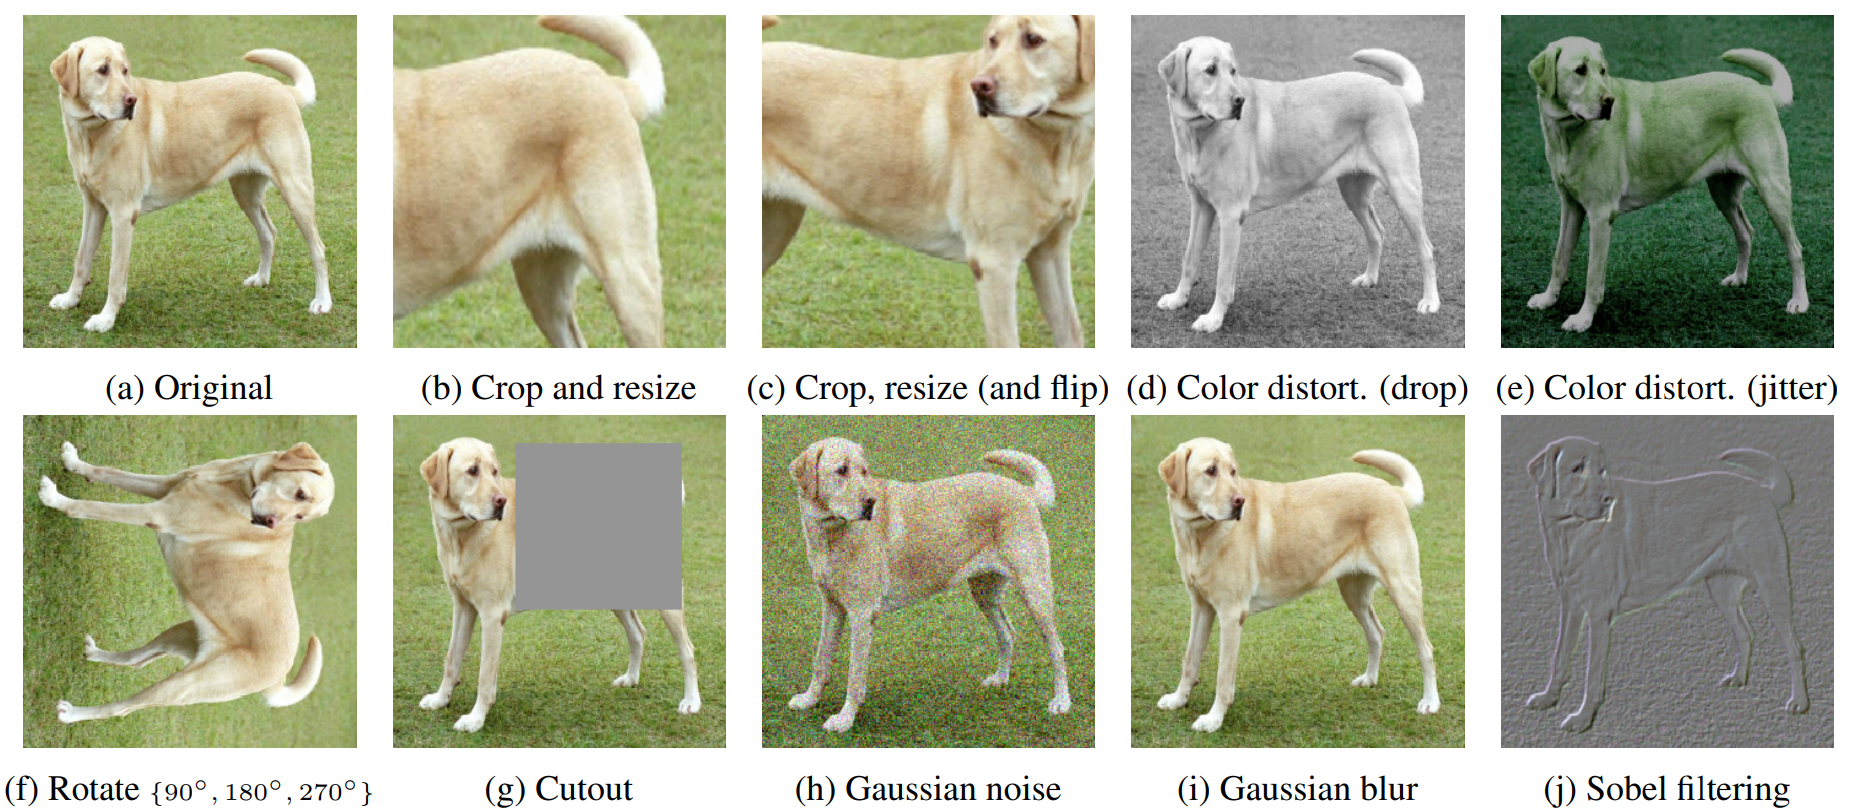
\includegraphics[scale=0.29]{images/Chapter2/example-data-augmentation.png}
    \caption[Ví dụ về việc áp dụng tăng cường dữ liệu lên hình ảnh]{Ví dụ về việc áp dụng tăng cường dữ liệu lên hình ảnh (Hình ảnh trích từ bài báo của Chen \cite{SimCLR}).}
\end{figure}

Việc áp dụng tăng cường dữ liệu lên văn bản cũng rất phổ biến. Ví dụ như thay thế bằng từ đồng nghĩa, xáo trộn câu. COCON \cite{CoCon} -- một kiến trúc mô hình được sử dụng phổ biến cho việc sinh ra dữ liệu dạng văn bản.

Trên đây là những khái niệm cơ bản và một số ví dụ về việc áp dụng phương pháp tăng cường dữ liệu. Ở các phần tiếp theo ta sẽ trình bày cụ thể hơn việc áp dụng tăng cường dữ liệu vào một bài toán cụ thể và việc áp dụng phương pháp này sẽ mang lại hiệu quả như thế nào đối với mô hình.

\section{Học tự giám sát} \label{2.4-ssl}

\noindent Đây sẽ là phần nền tảng cốt lõi nhất cho những thứ ta áp dụng sau này. Học tự giám sát (Self-supervised learning) \cite{ssl-genorcont, ssrl, survey:ssl-for-rec-sys, survey:ssl-from-perspectives, review:ssl-of-GNN} sẽ được sử dụng như là một phương pháp chung để giải quyết các bài toán và có thể áp dụng lên nhiều loại model. Ở phần này, ta sẽ giải thích các khái niệm cơ bản của học tự giám sát, vì sao người ta lại cần đến nó, cấu trúc tổng quát của nó như thế nào. 

\subsection{Học tự giám sát là gì?}

\noindent Việc áp dụng học giám sát để huấn luyện các mô hình học máy đã trở nên rất phổ biến và mang lại nhiều thành tựu to lớn từ trước đến nay. Các mô hình học sâu dần trở nên quá quen thuộc khi nhắc đến như Thị giác máy tính (Computer Vision), Xử lý ngôn ngữ tự nhiên (Natural Language Processing) hay gần đây thì có học đồ thị (Graph Learning). Tuy nhiên, ta nhận ra rằng các mô hình học sâu này luôn trong tình trạng ``đói dữ liệu'', thuật ngữ này đề cập đến vấn đề về kích thước mẫu cần thiết để mô hình học cho ra kết quả với độ chính xác đủ tốt. Với học giám sát, ta cần cung cấp cho mô hình một bộ dữ liệu đầu vào với cặp nhãn đi kèm. Với học không giám sát, ta chỉ cần cung cấp cho mô hình bộ dữ liệu không nhãn, mô hình sẽ học dựa trên cấu trúc của dữ liệu và dự đoán kết quả. Dù có áp dụng phương pháp nào, ta đều nhận thấy rằng khi ta cung cấp cho mô hình học càng nhiều dữ liệu, chất lượng đầu ra của mô hình có thể càng cải thiện. Vậy điều gì sẽ xảy ra khi ta chỉ có một tập dữ liệu có hạn? Lúc đó sẽ dễ dẫn đến trường hợp mô hình thiếu tính tổng quát hóa hay dẫn đến overfitting.

Tuy nhiên, khi xét về vấn đề dữ liệu trong bài toán học giám sát, ta biết rằng để có một bộ dữ liệu được gán nhãn đủ lớn thôi chưa đủ mà còn phải có chất lượng đủ tốt. Đây đã và đang là một vấn đề  còn vướng mắc và gặp rất nhiều hạn chế khi áp dụng trong các bài toán thực tế. Việc gán nhãn cho tập dữ liệu sẽ tốn rất nhiều chi phí, dữ liệu cũng có thể bị mất cân bằng hoặc thậm chí là không thể gán nhãn. Một bài toán nhận được kha khá sự quan tâm dạo thời gian đây với hi vọng giải quyết việc này là học tự giám sát (self-supervised learning). Phương pháp này nổi lên khá nhanh trong thời gian gần đây bởi khả năng áp dụng trên đa dạng loại dữ liệu từ âm thanh, hình ảnh, văn bản và đến cả đồ thị. Học tự giám sát sinh ra với khả năng giải quyết được vấn đề huấn luyện mô hình với phần lớn dữ liệu không được gán nhãn như đã đề cập ở trên. 

Học tự giám sát cho phép quá trình huấn luyện các mô hình học sâu bằng dữ liệu không dãn nhán hoặc một phần nhỏ được gán nhãn. Khi phải đối mặt với bộ dữ liệu không nhãn, học tự giám sát cho phép mô hình học được cách biểu diễn dữ liệu mà không cần gán nhãn dữ liệu bằng chính dữ liệu không nhãn. Khi phải đối mặt với bộ dữ liệu có số lượng nhãn hạn chế, học tự giám sát được áp dụng lên dữ liệu không dán nhãn đóng vai trò như một bước pre-train. Sau đó, sử dụng dữ liệu dán nhãn đã được sử dụng để fine-tune cho pretrain model.

Bên cạnh đó, học tự giám sát có thể  đóng vai là tác vụ phụ, có trách nhiệm bổ trợ cho task chính của mô hình. Áp dụng học tự giám sát không chỉ đạt được hiệu suất tương tự, một số trường hợp lại cho kết quả tốt hơn các mô hình học bởi phương thức có giám sát \cite{review:ssl-of-GNN}.

Mọi người thường nhầm lẫn giữa khái niệm học không giám sát và học tự giám sát. Học tự giám sát có thể được coi là một nhánh của học không giám sát. Vì cả hai đều hoạt động trên dữ liệu không nhãn. Tuy nhiên, học không giám sát chủ yếu hoạt động với các tác vụ phân cụm, gom nhóm, giảm chiều, trong khí đó học tự giám sát lại chủ yếu hoạt động với các tác vụ phân loại, hồi quy như học giám sát \cite{ssl-genorcont}.

Ở phần tiếp theo, ta sẽ giải thích kỹ hơn vì sao học tự giám sát lại quan trọng và được quan tâm trong thời gian gần đây

\subsection{Tại sao cần áp dụng học tự giám sát?} 

\noindent Việc tạo ra một tập dữ liệu tốt với đầy đủ nhãn là rất tốt kém về mặt chi phí lẫn thời gian. Trong khi ta bận tậm đến việc gán nhãn dữ liệu, thì dữ liệu không nhãn lại liên tục được sinh ra. Thay vì đầu tư vào việc gán nhãn, ta có thể tận dụng lượng lớn dữ liệu không nhãn sẵn có. Với học tự giám sát, mô hình có thể học được từ những đặc trưng chính từ bên trong của dữ liệu từ đó cải thiện độ chính xác của mô hình. 

Đi kèm với việc loại bỏ việc gán nhãn thủ công là khả năng mở rộng. Với lượng dữ liệu không nhãn được sinh ra mỗi ngày, dữ liệu sẽ ngày càng một lớn, sẽ rất khó nếu sử dụng các mô hình học giám sát. Thay vì đó, học tự giám sát có thể giải quyết được vấn đề khi không cần để tâm đến việc dữ liệu có nhãn hay không, càng nhiều dữ liệu không nhãn được sinh ra thì càng tốt. Và ắt hẳn điều này cũng giải quyết được việc mất cân bằng dữ liệu.

\subsection{Giới hạn của học tự giám sát?}

\noindent Không phải ngoại lệ, học tự giám sát mang lại nhiều lợi ích và tất nhiên cũng sẽ có một số điều hạn chế đi kèm. Ta cũng cần nắm rõ nhược điểm của học tự giám sát, từ đó tìm cách cải thiện, khắc phục nó.
Học tự giám yêu cầu chi phí sử dụng tài nguyên lớn. Học tự giám sát yêu cầu một lượng lớn dữ liệu, đồng thời cũng yêu cầu một lượng tài nguyên đủ lớn để xử lý được lượng dữ liệu đó. Cụ thể, mô hình cần hiểu được lượng dữ liệu to lớn mà nó được cung cấp, đồng thời tạo ra các nhãn tương ứng. Điều này sẽ tốn rất nhiều thời gian và tài nguyên so với các tác vụ học giám sát vì học tự giám sát được áp dụng khi dữ liệu đã có sẵn nhãn.

Khó giải thích sự hiệu quả mà học tự giám sát mang lại chưa chắc tốt. Mô hình tự học chính bên trong dữ liệu không nhãn mà nó được cung cấp, học được cách biểu diễn dữ liệu, học được các đặc trưng ẩn hữu dụng và ta không thể diễn giải được những điều đấy. Mô hình học tự giám sát sẽ tự động tạo ra các nhãn tương ứng với bộ dữ liệu mà nó được cung cấp mà không có bất kỳ sự hỗ trợ của con người. Điều này làm giảm các tác động dẫn đến lỗi sai của con người. Tuy nhiên, việc này có thể dẫn đến các lỗi sai lớn khi con người không trực tiếp giám sát điều này.

\subsection{Pretext Task and Downstream task}

\noindent Một khái niệm quan trọng trong Học tự giám sát là ``pretext task''.  Thuật ngữ này được dùng ở đây nhằm chỉ ra nhiệm vụ đang giải quyết không phải là vấn đề thật sự mà ta quan tâm, mục đích thực sự của nó là cung cấp cho ta một pre-train model đầy hứa hẹn. Những nhiệm vụ này có thể áp dụng được trên nhiều loại dữ liệu như hình ảnh, âm thanh, tín hiệu nhưng nhìn chung, pretext task có hai đặc điểm phổ biến. Một là mô hình có thể học được các đặc trưng có ích từ việc giải quyết các pretext task. Hai là các tín hiệu giám sát được tạo ra từ chính dữ liệu từ đó giúp mô hình có thể  học được tốt hơn \cite{survey:ssl-from-perspectives}.

Nói rõ hơn, trong học tự giám sát, trước tiên một pretext task sẽ cần được xác định, bên cạnh đó các nhãn giả cũng tự động sinh ra dựa trên một số thuộc tính nhất định của dữ liệu nhằm giúp các thuật toán học học sâu có thể giải quyết các pretext task đó. Sau khi quá trình pretrain này hoàn thành, mô hình học được có thể được sử dụng cho việc giải quyết các downstream task ví dụ như phân loại, phân cụm, phát hiện (cách này còn được gọi là transfer learning)

Hiện nay, có các loại pretext task phổ biến như context-based hay contrastive learning. Với phương thức context-based, có thể lấy việc xoay ảnh, đổi màu, thay đổi vị trí của các phần trong bức ảnh làm ví dụ. Với contrastive learning, ta có thể hiểu đơn giản việc áp dụng nhiệm vụ này có thể khiến các đối tượng gần giống nhau lại gần nhau, các đối tượng khác nhau ngày càng xa nhau trong không gian nhúng. Việc này sẽ nói rõ hơn ở phần dưới.
